\section{Existing Tools and Techniques}

\subsection{Imatest}
Imatest is a comprehensive software suite used for image quality testing developed by Imatest LLC\footnote[1]{https://www.imatest.com/}. It offers various modules to measure sharpness, noise, color accuracy, and other image quality factors using standardized test charts. Imatest's strengths lie in its extensive feature set and professional-grade accuracy. It is widely used in the industry by camera manufacturers, lens designers, and quality assurance teams. However, its complexity and cost can be prohibitive for amateur photographers.

Imatest employs a range of test charts and analytical techniques to evaluate lens performance. For example, it uses the SFRplus chart to measure spatial frequency response, which is crucial for assessing sharpness. The software also provides tools for analyzing distortion, chromatic aberration, and dynamic range. Despite its robustness, the steep learning curve and the need for specialized equipment make it less accessible to non-professional users \cite[]{ImatestAbout}.

\begin{figure}[h]
\centering
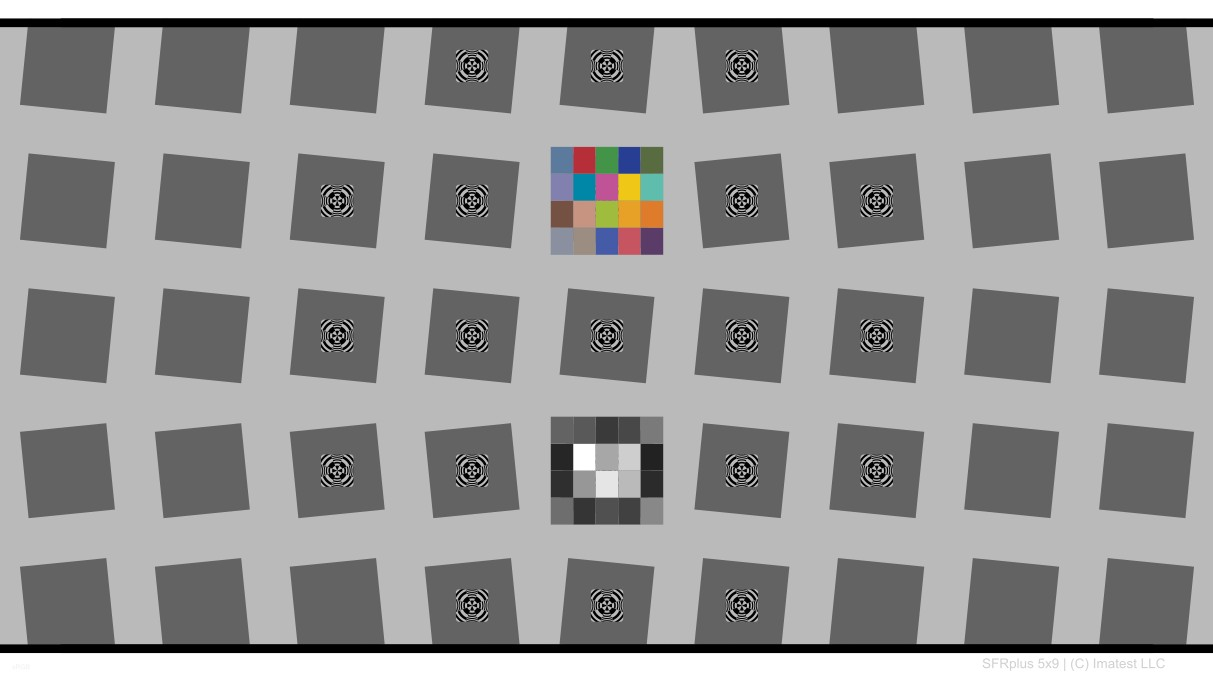
\includegraphics[height=5cm]{Images/SFRplus_chart.jpg}
\caption{Standard SFRplus test chart \cite{ImatestSFRChart}}
\label{fig:psf}
\end{figure}

\subsection{Dxomark}
Dxomark, a website by DXOMARK Image Labs\footnote[1]{https://www.dxomark.com/partners/}, provides image quality ratings for cameras, lenses, and mobile devices. Their tests include assessments of sharpness, exposure, color, noise, and optical distortions using standardized methodologies. Dxomark's ratings are industry-recognized and often cited by consumers and professionals alike when making purchasing decisions. The proprietary nature of its testing methods, however, limits user transparency and replicability \cite{DxomarkTestingLenses}.

Dxomark's lens testing protocol involves capturing images of various test scenes and charts under controlled conditions. They measure sharpness using a test chart with fine details and evaluate optical distortions by photographing grid patterns. Dxomark also assesses bokeh by analyzing images of defocused point light sources. While the results are comprehensive and reliable, the lack of detailed methodological disclosure means users cannot easily replicate the tests \cite{DxomarkBokeh}.

\subsection{Other Relevant Tools}
Beyond Imatest and Dxomark, several other tools and techniques are used for lens evaluation, including the Gletscherbruch Test and techniques measuring the sharpness and resolving power of an imaging system: the Edge Spread Function and the Line Spread Function.

\textbf{Gletscherbruch Test} evaluates decentering of a lens, which is a common issue where elements within the lens are not perfectly aligned, and can lead to blurriness and poor quality. The lens is first focused on a central target, then, without adjusting focus, the camera is moved to position the target in different corners of the frame. A decentered lens will show noticeable sharpness variations in different corners. \cite{Gletscherbruch}.

The \textbf{Edge Spread Function} (ESF) describes how a sharp edge is reproduced. It is a measure of the response of the imaging system to a high-contrast edge. Essentially, the ESF captures the transition from low to high intensity across the boundary of two areas. ESF is a critical for analyzing how sharp or blurred an edge appearsin an image.

The \textbf{Line Spread Function} (LSF) describes the response to a line. The LSF is derived from the ESF by taking its derivative. The LSF is a one-dimensional representation of how a thin line would appear when imaged by the system \cite{ESF}.

\section{Key Concepts in Optical Image Quality Evaluation}

\subsection{Point Spread Function (PSF)}
The Point Spread Function (PSF) describes how a point source of light is imaged by an optical system. It represents the system's response to a point source and is a critical factor in determining image sharpness. A smaller PSF indicates better resolving power and sharper images \cite{PSFdescription}.

\begin{figure}[h]
\centering
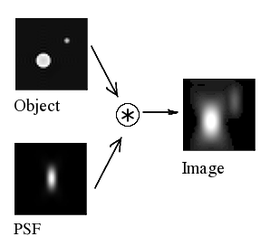
\includegraphics[width=2.7cm]{Images/psf.png}
\caption{Example of Point Spread Function \cite{PSF}}
\label{fig:psf}
\end{figure}

\subsection{Modulation Transfer Function (MTF)}
The Modulation Transfer Function (MTF) measures the ability of an optical system to reproduce (transfer) contrast from the subject to the image at various spatial frequencies. It is a crucial metric for assessing image sharpness. The MTF curve shows how contrast varies with spatial frequency, with higher values indicating better performance \cite{MTF}.

\begin{figure}[h]
\centering
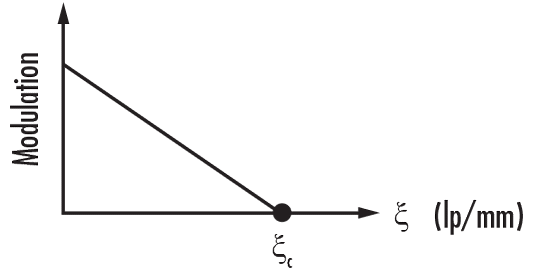
\includegraphics[height=3.5cm]{Images/MTF_example.png}
\caption{Example of Modulation Transfer Function for an Aberration-Free Lens with a Rectangular Aperture \cite{MTFimage}.}
\label{fig:mtf}
\end{figure}

\subsection{Optical Transfer Function (OTF)}
The Optical Transfer Function (OTF) combines the MTF and phase information to provide a complete description of the imaging system's performance. While the MTF only considers amplitude, the OTF includes both amplitude and phase, offering a more comprehensive view of how an optical system handles different spatial frequencies.

\begin{figure}[h]
\centering
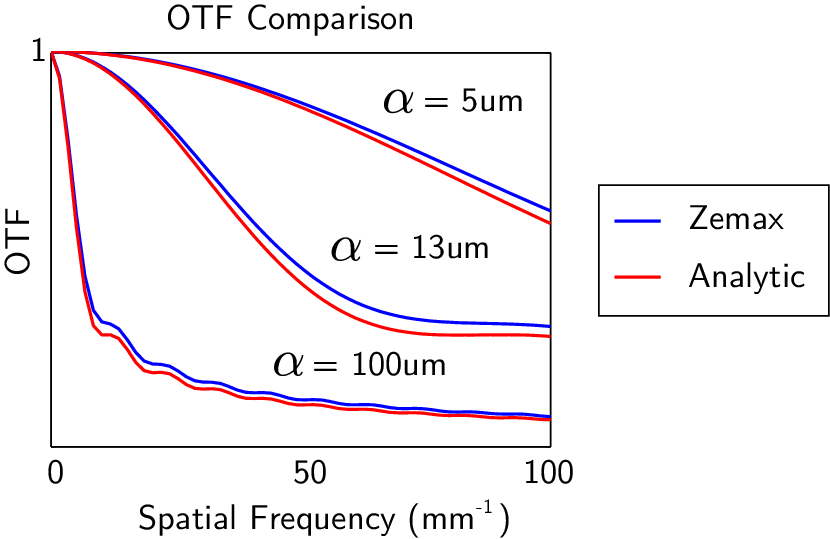
\includegraphics[height=5cm]{Images/OTF_example.png}
\caption{Example of Optical Transfer Function for a lens with spherical aberration \cite{OTFimage}}
\label{fig:otf}
\end{figure}

\section{Additional Concepts and Techniques}

\subsection{Accutance}
Accutance is a measure of perceived sharpness, taking into account both the contrast at edges and the human visual system's sensitivity to different spatial frequencies. It combines sharpness and contrast to provide a more comprehensive assessment of image quality \cite{accutance} .

\subsection{Sharpness and Optical Resolution}
Sharpness refers to the clarity and detail of an image, while resolution measures the amount of detail an imaging system can capture, typically in pixels. Higher resolution allows for larger prints and more detailed images.

\subsection{Geometric Distortions}
Image distortions occur when straight lines in an image get unnaturally curved or deformed. Distortions are caused by aberrations near the edges of the image and can result from the use of certain lenses. Common types of distortion include barrel distortion, where lines bulge outward, typically seen when a lens is at full zoom; pincushion distortion, where lines curve inward, frequently associated with telephoto lenses; and waveform distortion, a combination of both barrel and pincushion distortions, often occurring with wide-angle cameras in zoom mode \cite{distortions}.

\begin{figure}[htbp]
  \centering
  \begin{subfigure}[b]{0.45\textwidth}
    \centering
    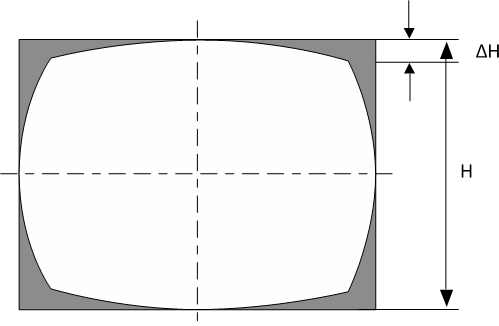
\includegraphics[height=3.3cm]{Images/barrel_distortion.png}
    \caption{Barrel distortion}
    \label{fig:barrel}
  \end{subfigure}
  \hfill
  \begin{subfigure}[b]{0.45\textwidth}
    \centering
    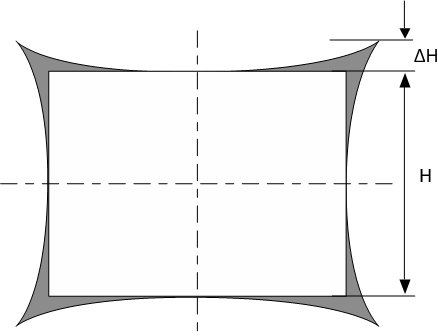
\includegraphics[height=3.3cm]{Images/pincushion_distortion.png}
    \caption{Pincushion distortion}
    \label{fig:pincushion}
  \end{subfigure}
  \caption{Examples of distortions \cite{distortions}.}
  \label{fig:distortions}
\end{figure}

\subsection{Chromatic Aberrations}
Chromatic aberration is an optical phenomenon caused by a lens failing to focus different wavelengths of light at the same point. There are two types of chromatic aberrations: longitudinal (axial), where different wavelengths of color do not converge at the same point after passing through a lens, and lateral, where different wavelengths of color coming at an angle focus at different positions along the same focal plane. Chromatic aberrations can degrade image quality and are typically corrected through lens design or software post-processing \cite{ChromaticAberation}.

\begin{figure}[h]
\centering
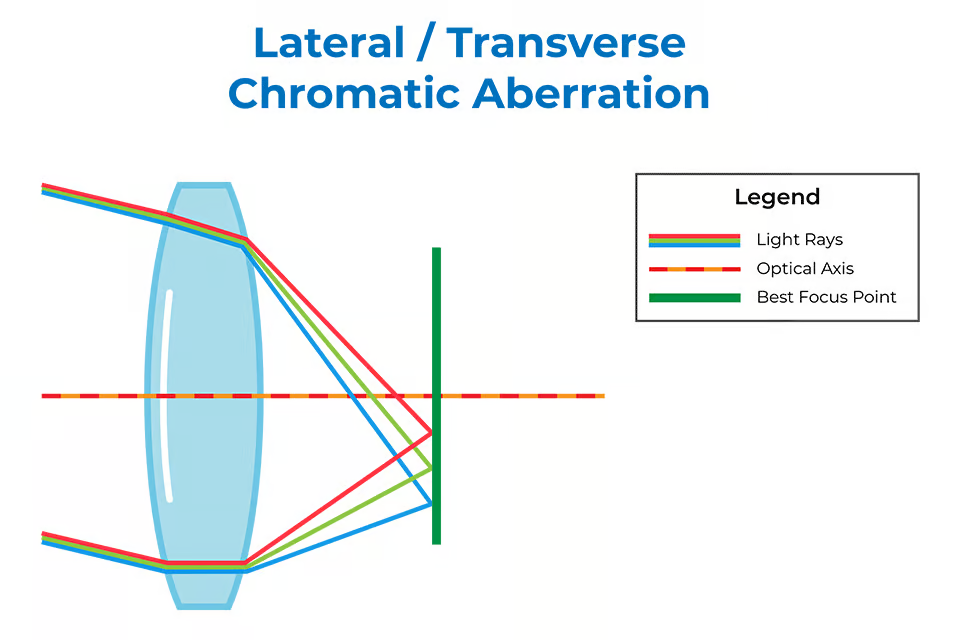
\includegraphics[height=4cm]{Images/chromatic_aberation.png}
\caption{Lens with lateral chromatic aberration \cite{ChromaticAberation}.}
\label{fig:chrom_ab}
\end{figure}

\begin{figure}[h]
\centering
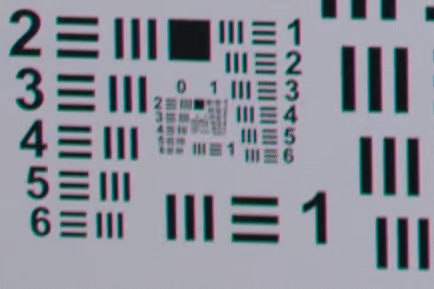
\includegraphics[height=2.9cm]{Images/chromatic_aberation_photo.png}
\caption{Example of a chromatic aberration \cite{ChromaticAberation}}
\label{fig:chrom_ab}
\end{figure}

\subsection{Bokeh}
Bokeh describes the aesthetic quality of the out-of-focus areas in an image, often characterized by the shape and smoothness of background blur produced by the lens. Bokeh depends on lens aperture shape and size as well as other lens characteristics.

\subsection{Airy Disk}
An Airy disk is the diffraction pattern produced by a circular aperture, representing the fundamental limit of resolution for optical systems. It appears as a central bright spot surrounded by concentric rings of decreasing intensity. The diameter of the Airy disk depends on the wavelength of the light and the size of the aperture. \cite{AiryDisk}.

\begin{figure}[htbp]
\centering
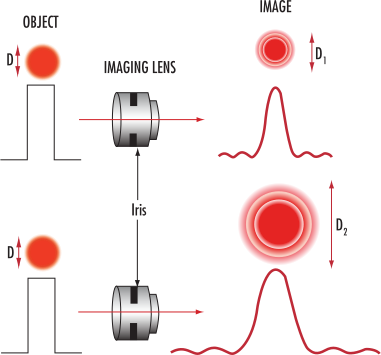
\includegraphics[height=5cm]{Images/airy_disk.png}
\caption{Airy disks depend on size of imaging lens aperture \cite{AiryDisk}}
\label{fig:airy_disk}
\end{figure}

\subsection{Aliasing}
Aliasing occurs when a signal is undersampled, causing different signals to become indistinguishable. Aliasing is related to maximum spatial frequency, called the Nyquist frequency. Any information above the Nyquist frequency that reaches the sensor will be aliased to a lower spatial frequency and create visual artifacts. In imaging, it manifests as jagged edges or moiré patterns, especially when capturing fine details \cite{Aliasing}.

\begin{figure}[htbp]
\centering
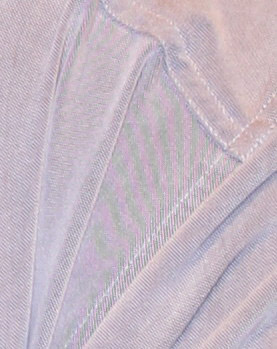
\includegraphics[height=5cm]{Images/color_moire.jpg}
\caption{Color Moiré pattern, an example of aliasing \cite{Aliasing}}
\label{fig:moire}
\end{figure}

\subsection{Focus Breathing}
Focus breathing refers to the change in a lens's field of view when adjusting focus, noticeable as a slight zooming effect during focusing \cite{FocusBreathing}.

\subsection{Test Charts}
Test charts are printed or digital patterns with known properties used to evaluate and calibrate the performance of imaging systems, assessing parameters like resolution, color accuracy, and distortion.

\subsection{Dynamic Range}
Dynamic range is the range of light intensities a camera can capture, from the darkest shadows to the brightest highlights. High dynamic range (HDR) imaging techniques are used to enhance detail in both dark and bright areas.

\subsection{Noise}
Noise refers to random variations in pixel values, often visible as graininess or speckles in an image. It is more pronounced in low-light conditions and high ISO settings.

\subsection{Color Accuracy}
Color accuracy measures how faithfully a camera reproduces colors compared to the original scene. It is critical for applications requiring precise color reproduction, such as product photography and medical imaging.

\section{Software Libraries and Tools}

\subsection{Camera Control Libraries}
\subsubsection{gphoto2}
The gphoto2 library provides a robust foundation for interfacing with digital cameras. It offers several key capabilities essential for lens testing including direct camera control through USB connections, remote capture capabilities, access to camera settings and configurations, support for multiple camera manufacturers, and RAW image capture support \cite{gphoto2}.

The library's architecture enables programmatic control of camera functions, making it possible to automate test sequences and ensure consistent capture conditions across multiple tests. The API provides both high-level functions for simple operations and low-level access for complex control requirements.

\subsection{Image Processing Libraries}
\subsubsection{OpenCV}
OpenCV (Open Source Computer Vision Library) serves as a cornerstone for lens analysis applications \cite{opencv}. Its capabilities include:
\begin{itemize}
    \item Advanced edge detection algorithms essential for MTF calculations
    \item Image filtering and noise reduction
    \item Geometric distortion analysis
    \item Color space conversions
    \item Efficient image manipulation routines
\end{itemize}

The library's optimized algorithms make it particularly suitable for real-time analysis of high-resolution images, a crucial requirement for lens testing applications.

\subsubsection{rawpy}
rawpy provides essential capabilities for working with RAW image files \cite{rawpy}. Its features include:
\begin{itemize}
    \item Direct access to sensor data
    \item Debayering algorithms
    \item Color space conversion
    \item Exposure adjustment
    \item White balance control
\end{itemize}

The ability to work with RAW files is crucial for lens testing as it provides access to unprocessed sensor data, enabling more accurate analysis of lens characteristics.

\subsection{Modern Web Frameworks}
\subsubsection{NiceGUI}
NiceGUI represents a new generation of Python web frameworks particularly suited for scientific applications \cite{nicegui}. Key features include:
\begin{itemize}
    \item Real-time updates without page refreshes
    \item Integration with Python data processing
    \item Modern reactive UI components
    \item Efficient handling of large datasets
    \item Built-in support for data visualization
\end{itemize}

\subsection{Testing Tools and Standards}
\subsubsection{Test Charts and Patterns}
Modern lens testing relies on standardized test patterns:
\begin{itemize}
    \item ISO 12233 resolution charts
    \item Siemens star patterns for MTF measurement
    \item Grid patterns for distortion analysis
    \item Dot patterns for chromatic aberration testing
    \item Greyscale gradients for vignetting analysis
\end{itemize}

These patterns provide standardized methods for measuring various lens characteristics, enabling consistent and comparable results.

\subsection{Analysis and Visualization Tools}
\subsubsection{Matplotlib}
Matplotlib provides essential visualization capabilities for lens testing \cite{matplotlib}:
\begin{itemize}
    \item MTF curve plotting
    \item Distortion map visualization
    \item Vignetting pattern display
    \item Interactive result exploration
    \item Publication-quality graph generation
\end{itemize}

\subsection{Integration and Automation Tools}
\subsubsection{Python Ecosystem}
The Python ecosystem offers several tools crucial for lens testing applications:
\begin{itemize}
    \item numpy for numerical computations \cite{numpy}
    \item scipy for scientific algorithms
    \item pandas for data organization
    \item PIL/Pillow for image handling
    \item logging for system monitoring
\end{itemize}

These tools together provide a comprehensive foundation for building sophisticated lens testing applications.

\subsection{Data Management and Organization}
Modern lens testing systems must handle various data formats:
\begin{itemize}
    \item RAW image formats (CR2, NEF, ARW)
    \item Standardized result formats
    \item Metadata storage
    \item Test configuration data
    \item Analysis results
\end{itemize}

The selection and implementation of appropriate data formats significantly impacts system usability and interoperability.

\subsection{Emerging Technologies}
Recent developments in machine learning are beginning to influence lens testing:
\begin{itemize}
    \item Automated pattern recognition
    \item Defect detection
    \item Quality prediction
    \item Test result classification
    \item Performance optimization
\end{itemize}

These technologies show promise in automating and improving the accuracy of lens testing procedures. The integration of these various tools and libraries enables the development of comprehensive lens testing solutions that can match or exceed the capabilities of traditional commercial systems while maintaining accessibility and ease of use.